% Source of report.pdf. Compile with ./build_report.sh (pdfLaTeX, two passes).
% Scientific results are reproduced in the notebooks and exported to reports/*.json.
\documentclass[10pt,a4paper]{article}
\usepackage[T1]{fontenc}
\usepackage[utf8]{inputenc}
\usepackage[english]{babel}
\usepackage{lmodern}
\usepackage{amsmath,amssymb}
\usepackage[top=1.8cm,bottom=1.8cm,left=2cm,right=2cm]{geometry}
\usepackage{microtype}
\usepackage{graphicx}
\usepackage{float}
\usepackage{booktabs,array}
\usepackage[font=small,labelfont=bf,justification=raggedright,singlelinecheck=false]{caption}
\usepackage[hidelinks]{hyperref}
\hypersetup{pdftitle={Explaining customer churn: an end-to-end XAI case study},
  pdfsubject={Explainable AI final project, Option A, academic year 2026/27},
  pdfauthor={Nicolás del Val}}
\urlstyle{same}
\linespread{1.08}
\setlength{\parindent}{0pt}
\setlength{\parskip}{0.45em}
\setlength{\emergencystretch}{2em}
\setlength{\textfloatsep}{12pt plus 2pt minus 2pt}
\setlength{\intextsep}{10pt plus 2pt minus 2pt}
\setcounter{topnumber}{3}
\setcounter{bottomnumber}{2}
\renewcommand{\topfraction}{0.9}
\renewcommand{\bottomfraction}{0.8}
\renewcommand{\textfraction}{0.1}
\renewcommand{\floatpagefraction}{0.8}
\providecommand{\tightlist}{\setlength{\itemsep}{0pt}\setlength{\parskip}{0pt}}
\title{\vspace{-1.5em}\Large\bfseries Explaining customer churn:\\an end-to-end XAI case study}
\author{Nicolás del Val}
\date{\small Explainable AI, final project (Option A), academic year 2026/27}
\begin{document}
\maketitle
\vspace{-1em}

\section{Introduction}\label{introduction}

A telecom retention team has a limited budget and must decide whom to
contact and which offer to investigate. A churn score supports
prioritisation; explanations help inspect the reasons behind that score
and identify potentially misleading recommendations. A second
stakeholder, the model auditor, needs to assess whether the predictions
depend on sensible signals and whether the explanations deserve trust.

Here I train and evaluate a model, compare explanations, test their
sensitivity and use them to simplify the model and examine retention
levers. The central
distinction is between explaining a prediction and establishing what
would actually retain a customer.

\section{Data and methods}\label{data-and-methods}

\subsection{Task and data}\label{task-and-data}

I classify the binary \texttt{Churn} label from a customer's
demographics, tenure, subscribed services, contract and billing profile.
The public IBM Telco Customer Churn sample \cite{ibm} contains 7,043
customers and 21 columns, with 26.5 \% churn. Dropping
\texttt{customerID} and the target leaves 19 features: four
numeric-coded columns (\texttt{SeniorCitizen}, \texttt{tenure},
\texttt{MonthlyCharges}, \texttt{TotalCharges}) and 15 text categorical
columns. \texttt{SeniorCitizen} is a binary indicator, not continuous
age. Observed churn is 42.7 \% for month-to-month, 11.3 \% for one-year
and 2.8 \% for two-year contracts.

\texttt{TotalCharges} contains 11 blanks, all at zero tenure; I encode
these not-yet-billed profiles as 0 and reject missing values at positive
tenure. This row-wise rule learns nothing from other customers. One-hot
encoding and numeric scaling for logistic regression are fitted inside
each training fold's pipeline. There are 22 duplicate feature-target
rows after removing the ID. I retain them because identical profiles
may represent different customers; their possible effect on evaluation
optimism is unquantified.

\subsection{Evaluation protocol and
models}\label{evaluation-protocol-and-models}

I use a stratified 80/20 split with seed 42: 5,634 training and 1,409
test customers. Five-fold inner CV selects hyperparameters on training
only; the reported CV estimate repeats the search within five outer
folds. I compare a constant-prior majority baseline, L2 logistic
regression (tuned \texttt{C}) and XGBoost (tuned depth and number of
trees). All fitted preprocessing is inside the pipelines. A
train-minus-CV AUC gap below 0.03 is my operational overfitting
diagnostic, not a universal guarantee of generalisation.

\textbf{Exploratory status.} The initial models are fitted and tuned
without test data. I subsequently inspect test explanations before
finalising the simplification hypothesis. Redundancy checks and
numerical variant selection use training data, but the later test
comparison is descriptive, not an untouched confirmatory evaluation.
Rechecking training evidence does not undo earlier test inspection.
Confirmation of the complete revised procedure requires an independent
cohort.

I report churn-class precision, recall, F1 and average precision
(called PR-AUC here), ROC-AUC and Brier score. No resampling or class
weighting is used. A missed churner is assumed to cost \emph{r} times a
wasted offer, with \emph{r} = 5 as in \cite{elattar2026}, and sensitivity at 2 and
10. The initial operating threshold minimises this expected
\textbf{classification-error cost} on nested out-of-fold training
predictions. This cost does not model campaign effectiveness or the cost
of every contact.

\subsection{Explainability and its
evaluation}\label{explainability-and-its-evaluation}

Option A uses three complementary techniques: \textbf{TreeSHAP},
\textbf{permutation importance} and \textbf{DiCE counterfactuals},
covering global and local questions. Logistic regression supplies a
separate interpretable reference.

TreeSHAP \cite{lundberg2017,lundberg2020} gives additive contributions to XGBoost's log-odds.
One-hot contributions are summed by original feature. Contributions are
centred on the average training log-odds; because the selected model
contains depth-1 trees, this is equivalent to interventional SHAP with
the same background. A check using 100 background customers differs by
at most 0.068 log-odds from the full-training reference. Global
importance is mean absolute contribution; local values explain one
customer's score. Permutation importance \cite{fisher2019} measures the drop in
ROC-AUC after shuffling an original feature. Logistic contributions are
coefficient times deviation from the average training customer. I
compare ranks across methods because AUC loss and log-odds have
different units.

I adapt the label-randomisation idea of Adebayo et al.~\cite{adebayo2018} to
tabular SHAP. Ten shuffled-label refits should have mean Spearman
correlation below 0.5 with the real importance ranking; ten bootstrap
refits retaining labels are the control. For deletion, training-derived
top-k rankings should produce an AUC loss above the 95th percentile of
reference k-feature subsets for each k = 1, 2, 3. These are diagnostic
criteria, not calibrated significance tests. After the exploratory audit
I strengthen the reference while retaining these criteria: enumerate
every singleton (50 permutations) and pair (10), and sample 200 distinct
triples without replacement (10). All rankings share the reference, and
an identical subset reuses its score. Reversed SHAP is a negative
control. The adopted model receives the same checks.

DiCE \cite{mothilal2020} proposes local profiles that cross the decision threshold.
I freeze non-actionable attributes, restrict possible changes to
billing, add-ons and contracts, and compare the proposals with
exhaustive search over the permitted combinations. A wrapper maps the
operating boundary to DiCE's 0.5 boundary; reported probabilities come
from the original model. Minimum change count is not minimum financial
cost or proof that a customer would accept the changes.

\section{Results}\label{results}

\subsection{Model performance and
decisions}\label{model-performance-and-decisions}

Table~\ref{tab:discrimination} shows small train-CV gaps, below my operational limit, and test
performance close to CV. This supports limited overfitting under the
evaluated protocol. XGBoost's mean CV AUC is numerically higher, but
comparing separate fold standard deviations is not a paired significance
test; I infer neither superiority nor equivalence from them. The
selected XGBoost has depth 1 and 600 trees: an additive model, best
within the tested grid rather than proof that interactions never matter.

\begin{table}[H]
\centering\small
\setlength{\tabcolsep}{4pt}
\begin{tabular*}{\linewidth}{@{\extracolsep{\fill}}lrrrrrr@{}}
\toprule
Model & Train AUC & CV AUC ($\pm$ sd) & Test AUC & Gap & CV PR-AUC & Test PR-AUC \\
\midrule
Majority class & 0.500 & 0.500 \ensuremath{\pm} 0.000 & 0.500 & 0.000 & 0.265 & 0.265 \\
Logistic regression & 0.850 & 0.846 \ensuremath{\pm} 0.013 & 0.841 & 0.004 & 0.661 & 0.628 \\
XGBoost & 0.859 & 0.851 \ensuremath{\pm} 0.012 & 0.848 & 0.008 & 0.672 & 0.670 \\
\bottomrule
\end{tabular*}
\caption{Discrimination. Train and CV scores use the
same outer-fold models. A constant score has PR-AUC equal to prevalence,
0.265.}
\label{tab:discrimination}
\end{table}

At \emph{r} = 5, both initial thresholds are 0.17, close to the
calibrated analytic boundary 1/(1+\emph{r}) = 0.167. Calibration is
checked directly on out-of-fold training predictions (Figure~\ref{fig:calibration}): the
largest of ten equal-count bin deviations is 0.045 for logistic
regression and 0.021 for XGBoost. This is finite-sample evidence, not
perfect calibration or proof that avoiding resampling caused it.

\begin{table}[H]
\centering\small
\setlength{\tabcolsep}{4pt}
\begin{tabular*}{\linewidth}{@{\extracolsep{\fill}}lrrrrrr@{}}
\toprule
Model & Precision & Recall & F1 & Accuracy & Brier & \shortstack[r]{Cost per\\customer} \\
\midrule
Majority (never flags) & 0.000 & 0.000 & 0.000 & 0.735 & 0.195 & 1.327 \\
Logistic regression & 0.450 & 0.898 & 0.600 & 0.682 & 0.139 & 0.426 \\
XGBoost & 0.456 & 0.882 & 0.602 & 0.690 & 0.134 & 0.435 \\
\bottomrule
\end{tabular*}
\caption{Test churn-class metrics at \emph{r} = 5 and
threshold 0.17. Contacting everybody costs 0.735; the models reduce
expected error cost by 42.0 \% and 40.8 \%.}
\label{tab:cost}
\end{table}

Accuracy alone favours the majority classifier, which finds no churners.
The models find 88--90 \%, with about 45 true churners per 100 contacts
versus 26.5 in the population. Against the better model-free policy,
expected error cost falls by 32--44 \% across the three ratios. A paired
bootstrap of test customers gives a logistic-minus-XGBoost cost interval
of \ensuremath{-}0.038 to 0.021 at \emph{r} = 5. No difference is detected for any
ratio; intervals including zero do not establish equivalence.

\begin{figure}[H]
\centering
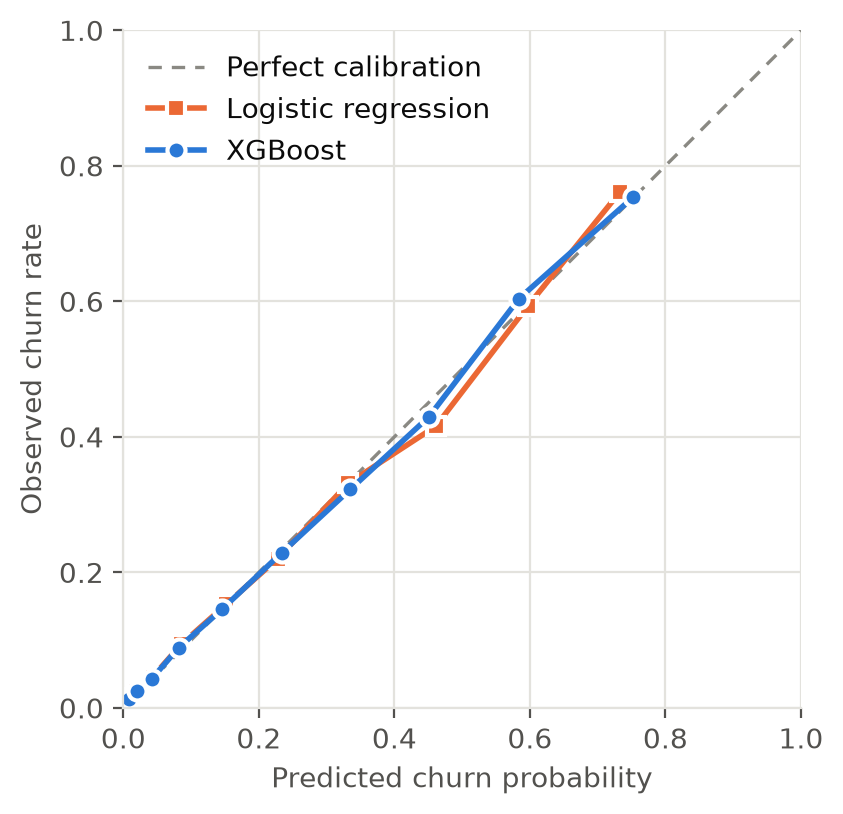
\includegraphics[width=0.46\textwidth,keepaspectratio]{figures/calibration.png}
\caption{Calibration on nested out-of-fold training
predictions (ten equal-count bins).}
\label{fig:calibration}
\end{figure}

\subsection{Global explanations}\label{global-explanations}

SHAP and permutation importance share Contract, tenure and
InternetService as their top three features; their rank correlation over
19 features is 0.83. Logistic regression shares two and correlates 0.79
with SHAP and 0.61 with permutation. The tail is noisy: several
permutation importances are indistinguishable within their shuffle
variability.

Figure~\ref{fig:importance} reveals informative disagreements. SHAP assigns Contract 19.4
\% of its total importance and tenure 17.6 \%, whereas permutation
assigns tenure 43.8 \% and Contract 29.4 \%. Logistic regression puts
MonthlyCharges first (22 \%). Services nearly reconstruct MonthlyCharges
(training CV \(R^2\) = 0.999), while its marginal churn correlation is +0.20
and its standardised logistic coefficient \ensuremath{-}1.97. Near-collinearity and
conditioning make a causal price interpretation unsafe. High
reconstruction \(R^2\) does not prove zero residual information; the ablation
below tests practical dispensability. Multiple correlated service
indicators may also split credit for the same profile characteristic.

\begin{figure}[H]
\centering
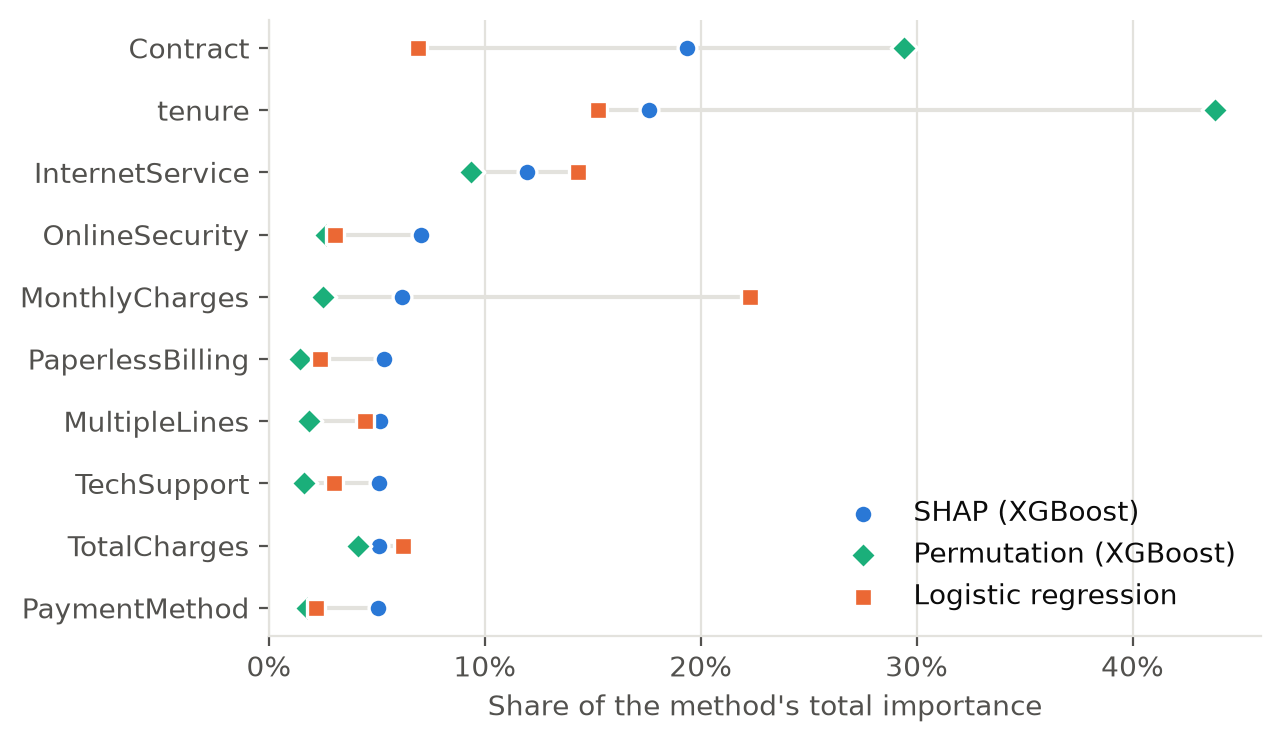
\includegraphics[width=0.72\textwidth,keepaspectratio]{figures/importance_by_method.png}
\caption{Ten leading features, each expressed as a
share of its own method's total importance. Shares do not make
magnitudes comparable across methods.}
\label{fig:importance}
\end{figure}

Tenure is nonlinear in XGBoost (Figure~\ref{fig:effects}): average contribution +1.48
log-odds at 0--1 months, +0.39 at 7--12, about zero at 13--24 and \ensuremath{-}0.48
at 49--71. The boundary at 72 months is not given a domain
interpretation. Month-to-month contracts contribute +0.55 versus \ensuremath{-}1.00
for two years; fibre optic contributes +0.42 versus \ensuremath{-}0.32 for DSL. These
describe the fitted model and differences between observed profiles.

\begin{figure}[H]
\centering
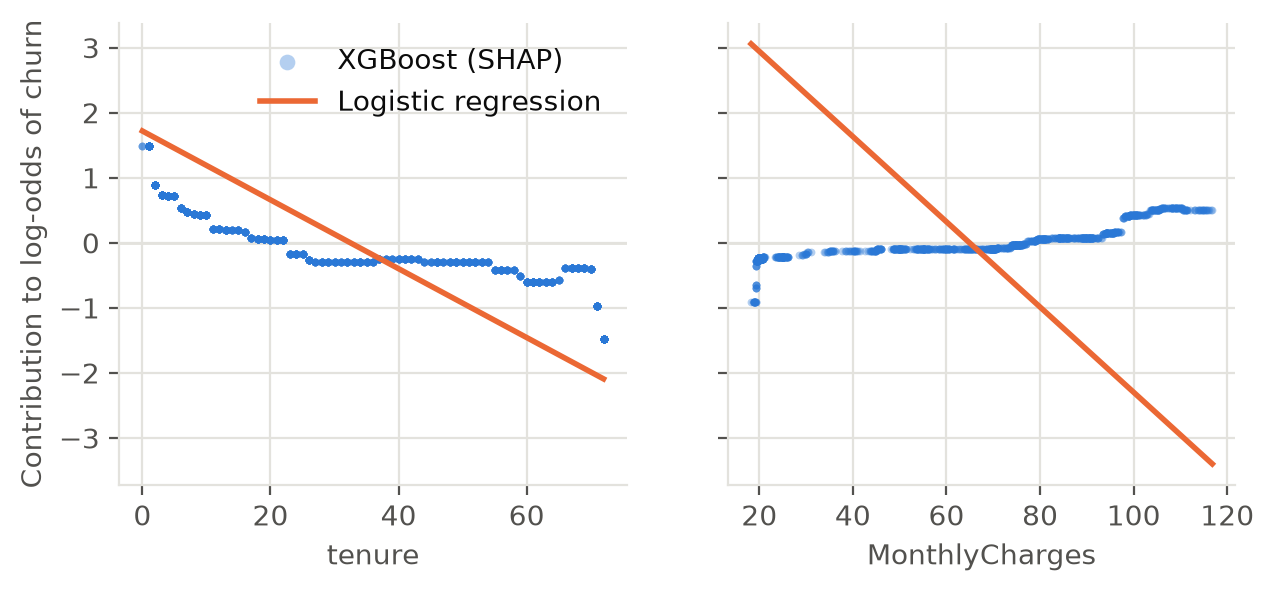
\includegraphics[width=0.72\textwidth,keepaspectratio]{figures/effects_numeric.png}
\caption{Contributions of tenure and MonthlyCharges:
XGBoost's nonlinear SHAP effects and logistic regression's linear
effects, in log-odds.}
\label{fig:effects}
\end{figure}

\subsection{Sanity checks of the initial
model}\label{sanity-checks-of-the-initial-model}

Label randomisation meets the diagnostic: mean Spearman 0.309, against
0.922 for bootstrap controls; one shuffled model has test AUC 0.517.
Total attribution falls to 0.46 from 3.12. The remaining correlation
warns that feature types and splitting opportunities can influence
rankings even without signal.

\textbf{The strengthened deletion reference overturns the earlier narrow
pass at k = 1.} SHAP's Contract-first ranking loses 0.0453 AUC, below
the singleton reference's 95th percentile, 0.0475. It exceeds the
strengthened reference at k = 2 and 3. Figure~\ref{fig:sanity} reports all three
rankings on XGBoost. SHAP and permutation select the same top-two and
top-three subsets and therefore receive identical deletion losses under
the shared perturbations. The complete all-k criterion is not passed by
SHAP. This is a useful limitation: attribution size and predictive
reliance are different quantities. Applying the logistic ranking to
XGBoost tests cross-model transfer, not the validity of logistic
explanations. Permutation importance is favoured because it targets the
metric used in the check.

\begin{figure}[H]
\centering
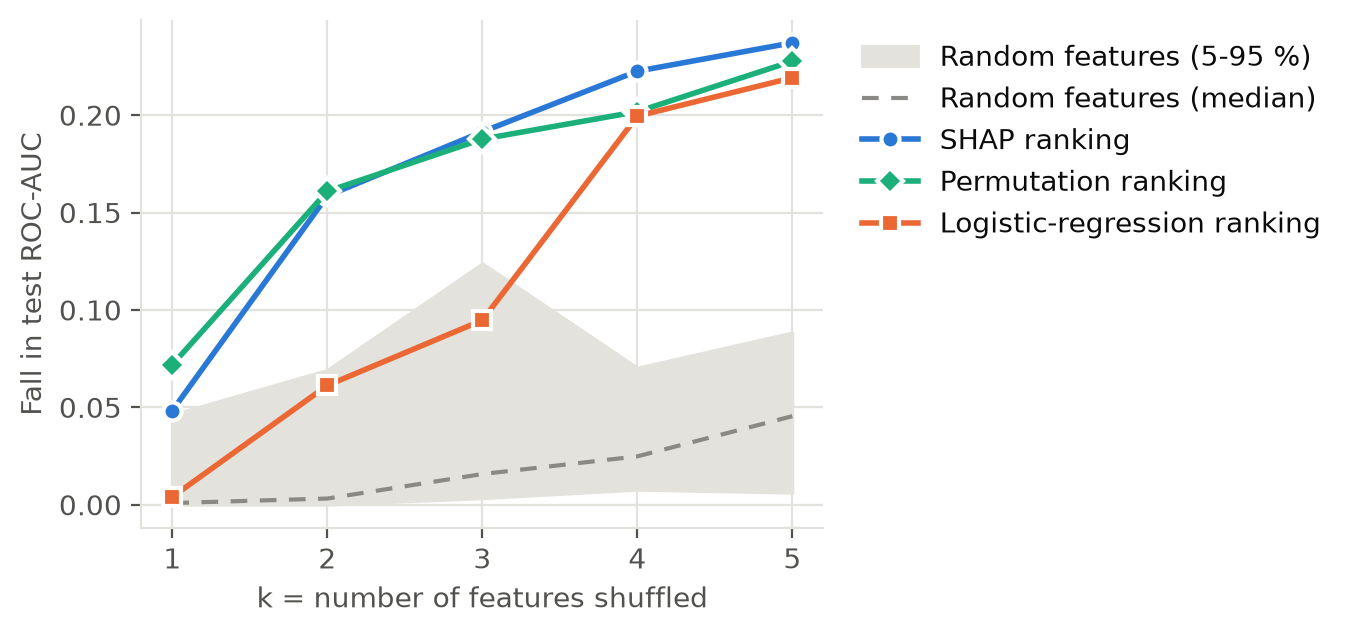
\includegraphics[width=0.76\textwidth,keepaspectratio]{figures/sanity_deletion.png}
\caption{AUC loss for training-derived rankings,
against distinct reference subsets: all 19 singletons and 171 pairs,
plus 200 sampled triples. The band is the 5--95 \% subset distribution,
not a confidence interval.}
\label{fig:sanity}
\end{figure}

\subsection{Local cases}\label{local-cases}

Figure~\ref{fig:local} uses the median-risk customer within each outcome group.
\textbf{A}, a flagged churner (P = 0.56), has positive contributions
from month-to-month contract (+0.55), fibre optic (+0.42), electronic
check (+0.23) and no online security (+0.22). \textbf{B}, a missed
churner (P = 0.10), has a two-year contract (\ensuremath{-}1.00), long tenure (\ensuremath{-}0.42)
and accumulated charges (\ensuremath{-}0.35) outweighing other signals. Complaints or
competing offers are plausible missing factors, but this error does not
demonstrate their cause: some churn is expected even at probability
0.10. \textbf{C}, a loyal customer flagged at P = 0.37, resembles
churners through contract and service profile. These explain model
scores, not customers' actual reasons.

\begin{figure}[H]
\centering
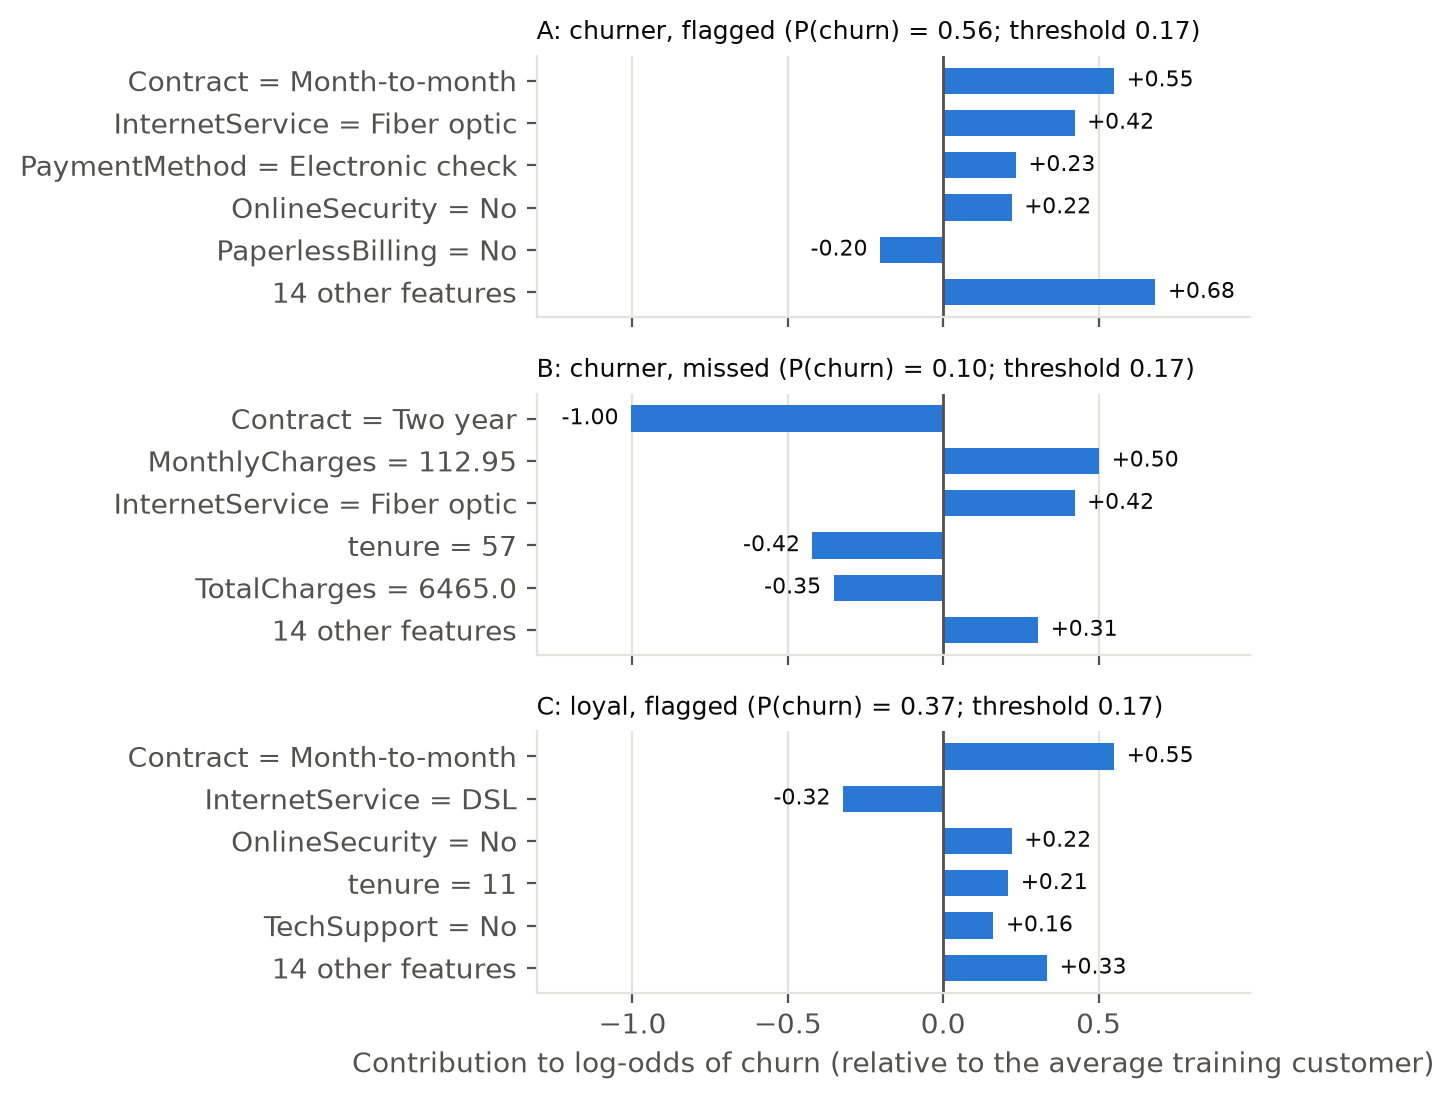
\includegraphics[width=0.82\textwidth,keepaspectratio]{figures/local_cases.png}
\caption{SHAP contributions for three representative
customers, relative to average training log-odds.}
\label{fig:local}
\end{figure}

\section{Actions and insights}\label{actions-and-insights}

\subsection{Simplification and validation of the adopted
model}\label{simplification-and-validation-of-the-adopted-model}

The explanations motivate removing MonthlyCharges and TotalCharges;
training CV reconstruction \(R^2\) is 0.999 for each (the latter from tenure,
monthly price and their product). I compare the original, either
removal and both removals using the same nested training folds. The
retained practical rule adopts the smallest version whose mean AUC loss
is at most 0.003 and mean error-cost increase at most 0.005. Both
removals qualify; removing TotalCharges alone exceeds the cost tolerance
(+0.0064). The paired CV AUC change for both is +0.0001 \ensuremath{\pm} 0.0013 (fold
standard deviation). Meeting mean tolerances is not a formal
non-inferiority test.

\begin{table}[H]
\centering\small
\setlength{\tabcolsep}{4pt}
\begin{tabular*}{\linewidth}{@{\extracolsep{\fill}}lrrrrrrr@{}}
\toprule
Version & Features & CV AUC & Test AUC & \shortstack[r]{Train--CV\\gap} & \shortstack[r]{Test\\PR-AUC} & Cost & Stability \\
\midrule
Before & 19 & 0.8508 & 0.8481 & 0.0082 & 0.670 & 0.4329 & 0.882 \\
After & 17 & 0.8509 & 0.8482 & 0.0053 & 0.669 & 0.4365 & 0.894 \\
\bottomrule
\end{tabular*}
\caption{Exploratory before/after comparison. Both use
the analytic threshold 1/(1+5), fixed independently of the comparison
folds; Table~\ref{tab:cost} uses the OOF-selected 0.17. Stability is mean Spearman
between eight bootstrap-refit rankings on 17 shared
features.}
\label{tab:improvement}
\end{table}

The gain is simplicity with essentially retained discrimination under
the selected tolerances. Test cost rises slightly. Stability rises from
0.882 to 0.894, but eight refits without an uncertainty interval do not
establish an improvement. Attribution is reallocated: removing redundant
price variables changes which remaining features receive credit.

I now test the adopted model's explanations, without using the verdicts
to choose another variant. Label-shuffle mean Spearman is 0.354 versus
0.932 for ten bootstrap controls. Table~\ref{tab:checks} uses the same strengthened
deletion protocol, with 17 singletons, 136 pairs and 200 distinct
triples. The adopted model meets both the label-randomisation criterion
and the deletion criterion for all three k values. Reversed SHAP does
not meet the criterion. This supports sensitivity to learned signal and
alignment with AUC reliance; it does not validate local directions,
causal actions or every aspect of explanation quality.

\begin{table}[H]
\centering\small
\setlength{\tabcolsep}{4pt}
\begin{tabular*}{\linewidth}{@{\extracolsep{\fill}}lrrrr@{}}
\toprule
Model & \shortstack[r]{Shuffled-label\\$\rho$} & \shortstack[r]{$k=1$\\loss / $q_{95}$} & \shortstack[r]{$k=2$\\loss / $q_{95}$} & \shortstack[r]{$k=3$\\loss / $q_{95}$} \\
\midrule
Initial (19) & 0.309 & 0.0453 / 0.0475 & 0.1510 / 0.0662 & 0.1882 / 0.0838 \\
Adopted (17) & 0.354 & 0.0960 / 0.0560 & 0.1863 / 0.0954 & 0.2369 / 0.1112 \\
\bottomrule
\end{tabular*}
\caption{SHAP diagnostics before and after
simplification. Each k cell compares AUC loss with its reference's 95th
percentile; every k must exceed it. Label randomisation requires mean
rho \textless{} 0.5. Subset coverage can be exhaustive while permutation
estimates remain noisy.}
\label{tab:checks}
\end{table}

\subsection{Prioritisation and candidate
levers}\label{prioritisation-and-candidate-levers}

At the adopted model's analytic threshold, 51 \% of customers are
flagged. With a smaller budget, the top 10 \% reaches 29 \% of churners
(77 \% churn within that group, 2.9 times prevalence), the top 20 \%
reaches 51 \%, and the top 30 \% reaches 66 \%. This concentrates risk,
not measured responsiveness to offers.

For 611 flagged month-to-month customers with internet service (43 \% of
the test sample), exhaustive search finds the fewest permitted profile
changes that lower the predicted score below threshold. Billing and
add-ons alone yield solutions for 156 customers. Longer contracts
dominate the broader scenarios (Table~\ref{tab:levers}); a contract change alone
suffices for 49 \% of the pool when two-year commitment is allowed.
Switching paperless billing off occurs in 118 of the 156 solutions
without a new contract: its apparent protection is an association
requiring investigation, not established intervention effectiveness.

\begin{table}[H]
\centering\small
\setlength{\tabcolsep}{4pt}
\begin{tabular*}{\linewidth}{@{\extracolsep{\fill}}lrrr@{}}
\toprule
Levers allowed & \shortstack[r]{Below the\\threshold} & \shortstack[r]{One change\\is enough} & \shortstack[r]{Mean risk\\before $\rightarrow$ after} \\
\midrule
Add-ons and billing only & 26 \% & 7 \% & 0.28 \ensuremath{\rightarrow} 0.15 \\
+ contract up to one year & 70 \% & 18 \% & 0.41 \ensuremath{\rightarrow} 0.14 \\
+ contract up to two years & 92 \% & 49 \% & 0.47 \ensuremath{\rightarrow} 0.12 \\
\bottomrule
\end{tabular*}
\caption{Model counterfactuals, not observed
retention. Each row averages its own solvable customers, so these risks
concern different cohorts.}
\label{tab:levers}
\end{table}

For two median-risk examples, all six DiCE proposals include a two-year
contract and match the exhaustive minimum change counts (two and three).
This demonstrates the method on those cases, not population-wide DiCE
optimality. Customer consent and feasible offer costs remain unmodelled.

On the same 156-customer cohort, modelled risk falls by 0.135, 0.156 and
0.207 across the three scenarios. If entirely causal, intervention cost
\emph{c} would break even at customer value \emph{V} \textgreater{} 7.4
\emph{c}, 6.4 \emph{c} and 4.8 \emph{c}; at one-quarter causal,
approximately 30 \emph{c}, 26 \emph{c} and 19 \emph{c}. These are
hypothetical sensitivity bounds, not estimated savings. Costs differ
between scenarios.

\section{Discussion}\label{discussion}

\textbf{Explanation reliability.} The initial singleton failure is
retained, not hidden by changing its threshold. Exhaustive
singleton/pair references remove subset-sampling uncertainty there, but
finite permutation noise remains and triples are sampled. Independent
shuffling can create implausible combinations of correlated services;
retained proxies can compensate for shuffled features. Agreement or a
pass does not establish correct attribution magnitudes, signs, local
stability or causality.

\textbf{Risk is not treatment benefit.} A long contract or
paperless-billing setting may mark loyal customers rather than cause
loyalty. High reconstruction \(R^2\) and attribution correlations do not
identify causal mechanisms. Retention depends on an offer's effect, not
only baseline risk \cite{ascarza2018}; one field experiment increased churn from 6
\% to 10 \% through proactive plan recommendations \cite{ascarza2016}. The
practical next step is a randomised pilot on eligible flagged customers,
measuring churn and costs against a control before recommending
deployment.

\textbf{Scope and confirmation.} Initial fitting and tuning use training
only, but the simplification follows inspection of test explanations and
its test comparison remains exploratory. No temporal split, future
lead-time validation or drift assessment is possible without dates. A
telecom study's AUC fell from 93.3 \% to 89 \% on later customers
\cite{ahmad2019}, motivating periodic re-evaluation. I have not measured
fairness across groups, despite demographic variables and possible
proxies. Independent prospective data, subgroup checks, offer acceptance
and causal uplift are needed before operational use.


\clearpage
\begin{thebibliography}{99}
\small\raggedright
\bibitem{elattar2026}
A. El Attar and M. El-Hajj, ``Explainable AI-driven customer churn
  prediction: a multi-model ensemble approach with SHAP-based feature
  analysis,'' \emph{Frontiers in Artificial Intelligence}, vol.~9, art.
  1748799, 2026.

\bibitem{ibm}
IBM, ``Telco Customer Churn'' sample data set,
  \url{https://raw.githubusercontent.com/IBM/telco-customer-churn-on-icp4d/master/data/Telco-Customer-Churn.csv}.

\bibitem{lundberg2017}
S. M. Lundberg and S.-I. Lee, ``A Unified Approach to Interpreting
  Model Predictions,'' \emph{Advances in Neural Information Processing
  Systems 30 (NeurIPS 2017)}, 2017.

\bibitem{lundberg2020}
S. M. Lundberg, G. Erion, H. Chen \emph{et al.}, ``From local
  explanations to global understanding with explainable AI for trees,''
  \emph{Nature Machine Intelligence}, vol.~2, pp.~56-67, 2020.
  doi:10.1038/s42256-019-0138-9.

\bibitem{fisher2019}
A. Fisher, C. Rudin and F. Dominici, ``All Models are Wrong, but Many
  are Useful: Learning a Variable's Importance by Studying an Entire
  Class of Prediction Models Simultaneously,'' \emph{J. Mach. Learn.
  Res.}, vol.~20, 2019. \url{https://jmlr.org/papers/v20/18-760.html}

\bibitem{adebayo2018}
J. Adebayo, J. Gilmer, M. Muelly, I. Goodfellow, M. Hardt and B. Kim,
  ``Sanity Checks for Saliency Maps,'' \emph{Advances in Neural
  Information Processing Systems 31 (NeurIPS 2018)}, 2018.
  arXiv:1810.03292.

\bibitem{mothilal2020}
R. K. Mothilal, A. Sharma and C. Tan, ``Explaining Machine Learning
  Classifiers through Diverse Counterfactual Explanations,'' \emph{Proc.
  ACM FAT* 2020}, 2020. arXiv:1905.07697.

\bibitem{ascarza2016}
E. Ascarza, R. Iyengar and M. Schleicher, ``The Perils of Proactive
  Churn Prevention Using Plan Recommendations: Evidence from a Field
  Experiment,'' \emph{J. Marketing Research}, vol.~53, no. 1, pp.~46-60,
  2016.

\bibitem{ascarza2018}
E. Ascarza, ``Retention Futility: Targeting High-Risk Customers Might
  be Ineffective,'' \emph{J. Marketing Research}, 2018.

\bibitem{ahmad2019}
A. K. Ahmad, A. Jafar and K. Aljoumaa, ``Customer churn prediction in
  telecom using machine learning in big data platform,'' \emph{J. Big
  Data}, vol.~6, art. 28, 2019. doi:10.1186/s40537-019-0191-6.
\end{thebibliography}

\end{document}
